\begin{figure}[ht]
	\centering
	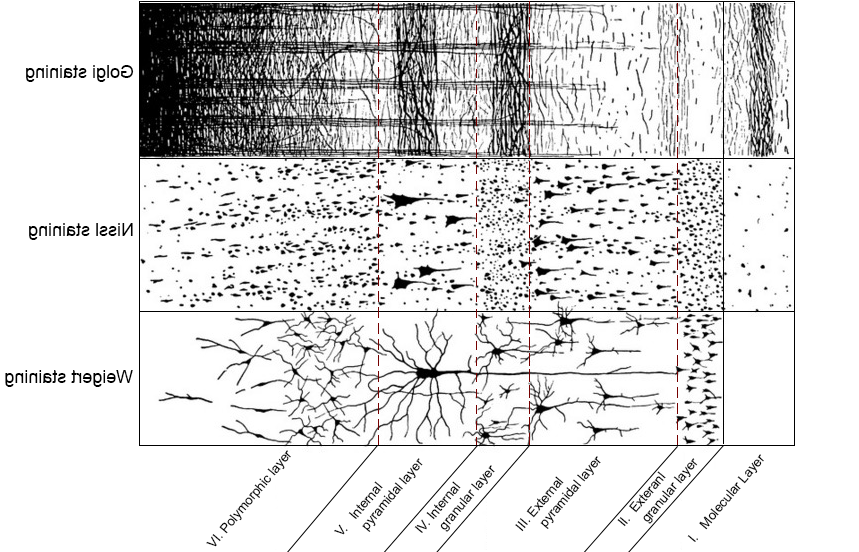
\includegraphics[width=0.8\textwidth, clip=true]{./Chapters/01_Introduction/Images/Layers}
	\caption{Cortical stainings of the histological layers, taken from Brodmann (1909) \cite{Brodmann1909}. Brodmann divided the cortex into regions, based on their differences in laminar structure. There is a wide variety in the thicknesses of the (sub)layers for different properties (nervous tissue, number of cell bodies, myelination), which can be highlighted with different stainings.}
	\label{fig:layers}
\end{figure}